%%%%%%%%%%%%%%%%%%%%%%% 用例分析 %%%%%%%%%%%%%%%%%%%%%%%%%%%%%%%%%%%%%%%%%%%%%
\chapter{用例分析}
	
\section{补充用例规约}
	经过讨论,上文中的用例已经足够详细了,此部分不添加用例规约。
\section{用例中类的析取}
    在第一章给出的用例归约的基础上,我们将挑选其中比较常用和重要的用例来分析,并给出用例的流程图。
    
	\subsection{用户注册用例分析} % (fold)
	\label{sub:用户注册用例分析}
	\begin{enumerate}
		\item \textbf{类的析取} \\
		用户注册用例允许微供应商和采购商在注册页面进行注册,其中包括的实体类、控制类和边界类如下图
		\autoref{fig:class_enroll}。
		\begin{figure}[htp]
		    %\begin{adjustwidth}{-1.5cm}{-1cm}
		    \centering
		    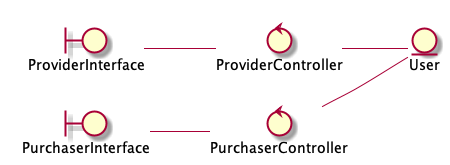
\includegraphics[width=12cm]{report/figure/classAnalyse/enroll.png}
		    \caption{注册用例析取图}
		    \label{fig:class_enroll}
		    %\end{adjustwidth}
		\end{figure}

		\item \textbf{用例工作时序图} \\
		注册用例需要用户在前端打开注册页面,填写信息后通过前端发送给后端,后端进行数据库操作后返回结果,具体流程如下图所示。正确的返回结果应该是待审核或注册失败。义微供应商的注册过程为例,其注册用例实现细节可见\autoref{fig:sd_enroll}。

		\begin{figure}[htp]
		    %\begin{adjustwidth}{-1.5cm}{-1cm}
		    \centering
		    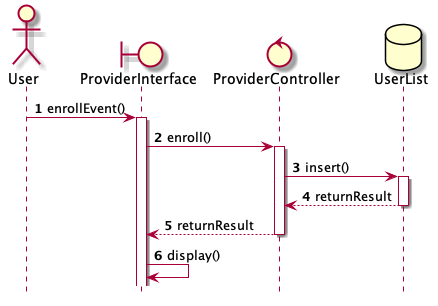
\includegraphics[width=12cm]{report/figure/sequenceDiagram/sd_enroll.png}
		    \caption{用户注册用例工作时序图}
		    \label{fig:sd_enroll}
		    %\end{adjustwidth}
		\end{figure}

	\end{enumerate}
	% subsection 用户注册用例分析 (end)

    \newpage
	\subsection{用户登录用例分析} % (fold)
	\label{sub:用户登录用例分析_name}
	\begin{enumerate}
		\item \textbf{类的析取} \\
		用户登录用例允许管理员、微供应商和采购商这三个类型的用户在登录页面进行登录,其中包括的实体类、控制类和边界类如下图
		\autoref{fig:class_login}.
		\begin{figure}[htp]
		    %\begin{adjustwidth}{-1.5cm}{-1cm}
		    \centering
		    
\includegraphics[width=12cm]{report/figure/classAnalyse/login.png}
		    \caption{用户登录用例析取图}
		    \label{fig:class_login}
		    %\end{adjustwidth}
		\end{figure}
		\item \textbf{登录用例时序图} \\
		登录用例需要用户在前端打开注册页面,填写信息后通过前端发送给后端,后端进行数据库操作后返回结果,具体流程如下图所示\autoref{fig:sd_login}。

		\begin{figure}[htp]
		    %\begin{adjustwidth}{-1.5cm}{-1cm}
		    \centering
		    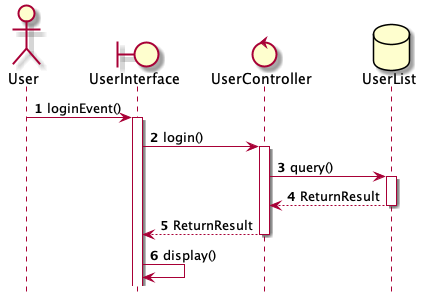
\includegraphics[width=12cm]{report/figure/sequenceDiagram/sd_login.png}
		    \caption{用户登录用例工作时序图}
		    \label{fig:sd_login}
		    %\end{adjustwidth}
		\end{figure}
	\end{enumerate}
	
	% subsection subsection_用户登录用例分析 (end)

% 	\subsection{发布母订单用例分析} % (fold)
% 	\label{sub:发布母订单用例分析}
% 	\begin{enumerate}
% 		\item \textbf{类的析取} \\
% 		发布母订单用例允许采购商进行母订单发布,其中包括的实体类、控制类和边界类如下图。
% 		\autoref{fig:class_apply}
% 		\begin{figure}[htp]
% 		    %\begin{adjustwidth}{-1.5cm}{-1cm}
% 		    \centering
% 		    
\includegraphics[width=12cm]{misc/figure_src/class_diagram/apply.png}
% 		    \caption{登录用例析取图}
% 		    \label{fig:class_apply}
% 		    %\end{adjustwidth}
% 		\end{figure}

% 		\item \textbf{用例工作时序图} \\ 
% 		发布母订单用例需要采购商登录后,点击发起母订单按钮,填写母订单信息后通过前端发送给后端,后端进行数据库操作后返回结果,正确的返回信息为待审核,具体流程如下图所示\autoref{fig:sd_generate}。

% 		\begin{figure}[htp]
% 		    %\begin{adjustwidth}{-1.5cm}{-1cm}
% 		    \centering
% 		    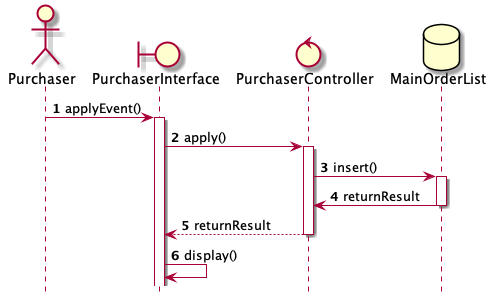
\includegraphics[width=12cm]{misc/figure_src/sequence_diagram/sd_applyMainOrder.png}
% 		    \caption{用户注册用例时序图}
% 		    \label{fig:sd_generate}
% 		    %\end{adjustwidth}
% 		\end{figure}

% 	\end{enumerate}
% 	% subsection 发布母订单用例分析 (end)
    \newpage
	\subsection{查看母订单用例分析} % (fold)
	\label{sub:查看母订单用例分析}
	\begin{enumerate}
		\item \textbf{类的析取} \\
		登录用例允许管理员、微供应商和采购商这三个类型的用户进行母订单相关查询,其中包括的实体类、控制类和边界类如下图
		\autoref{fig:class_queryMainOrder}。
		\begin{figure}[htp]
		    %\begin{adjustwidth}{-1.5cm}{-1cm}
		    \centering
		    
\includegraphics[width=12cm]{report/figure/classAnalyse/queryMainOrder.png}
		    \caption{查看母订单用例析取图}
		    \label{fig:class_queryMainOrder}
		    %\end{adjustwidth}
		\end{figure}

		\item \textbf{用例工作时序图} \\
		查看母订单用例需要用户登录后,在端点击“母订单查询”并填写相应信息后,将查询信息发送到后端,在后端进行数据库操作后返回结果,具体流程如下图所示\autoref{fig:sd_queryMainOrder}。

		\begin{figure}[htp]
		    %\begin{adjustwidth}{-1.5cm}{-1cm}
		    \centering
		    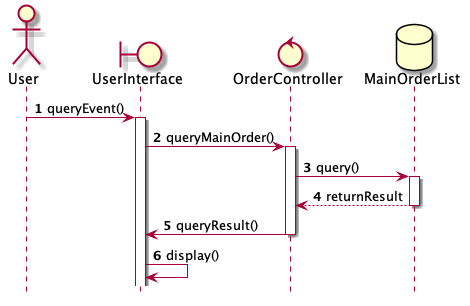
\includegraphics[width=12cm]{report/figure/sequenceDiagram/sd_queryMainOrder.png}
		    \caption{查看母订单用例工作时序图}
		    \label{fig:sd_queryMainOrder}
		    %\end{adjustwidth}
		\end{figure}

	\end{enumerate}
	
	% subsection 查看母订单用例分析 (end)

% 	\subsection{提交子订单用例分析} % (fold)
% 	\label{sub:提交子订单用例分析}
% 	\begin{enumerate}
% 		\item \textbf{类的析取} \\
% 		提交子订单用例允许微供应商在加入某个母订单并且通过审查后在相应子订单上更新自己的完成进度,其中包括的实体类、控制类和边界类如下图。
% 		\autoref{fig:class_commit}
% 		\begin{figure}[htp]
% 		    %\begin{adjustwidth}{-1.5cm}{-1cm}
% 		    \centering
% 		    
\includegraphics[width=12cm]{misc/figure_src/class_diagram/commit.png}
% 		    \caption{登录用例析取图}
% 		    \label{fig:class_commit}
% 		    %\end{adjustwidth}
% 		\end{figure}

% 		\item \textbf{用例工作时序图} \\
% 		在提交子订单用例中,微供应商填写进度信息等更新信息,由前端发送到后端,再在后端进行数据暂存等待管理员审核后返回相应的执行结果。具体流程如下图所示\autoref{fig:sd_commit}。

% 		\begin{figure}[htp]
% 		    %\begin{adjustwidth}{-1.5cm}{-1cm}
% 		    \centering
% 		    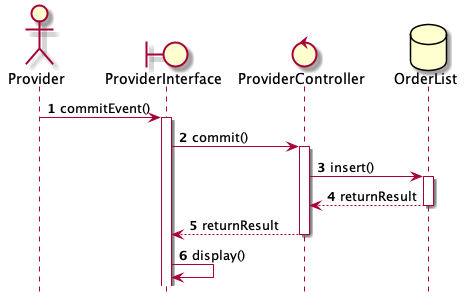
\includegraphics[width=12cm]{misc/figure_src/sequence_diagram/sd_commitOrder.png}
% 		    \caption{用户注册用例时序图}
% 		    \label{fig:sd_commit}
% 		    %\end{adjustwidth}
% 		\end{figure}

% 	\end{enumerate}
% 	% subsection 提交子订单用例分析 (end)

    \newpage
	\subsection{查看子订单用例分析} % (fold)
	\label{sub:查看子订单用例分析}
	\begin{enumerate}
		\item \textbf{类的析取} \\
		查看子订单用例允许管理员、微供应商和采购商在各自权限下查询子订单,其中包括的实体类、控制类和边界类如下图\autoref{fig:class_commit}。
		\begin{figure}[htp]
		    %\begin{adjustwidth}{-1.5cm}{-1cm}
		    \centering
		    
\includegraphics[width=12cm]{report/figure/classAnalyse/querySubOrder.png}
		    \caption{查看子订例析取图}
		    \label{fig:class_commit}
		    %\end{adjustwidth}
		\end{figure}

		\item \textbf{查看子订用例工作时序图} \\
		在查看子订单用例中,用户在前端填写查询信息,由端发送到后端,后端进行数据库操作后得到结果返回前端。具体流程如下图所示\autoref{fig:sd_querySubOrder}。

		\begin{figure}[htp]
		    %\begin{adjustwidth}{-1.5cm}{-1cm}
		    \centering
		    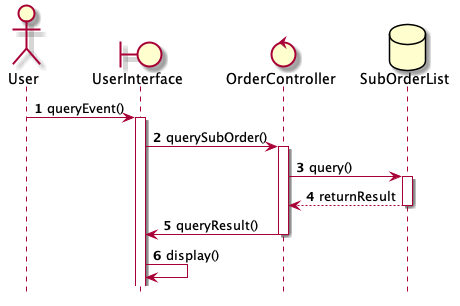
\includegraphics[width=12cm]{report/figure/sequenceDiagram/sd_querySubOrder.png}
		    \caption{查看子订用例工作时序图}
		    \label{fig:sd_querySubOrder}
		    %\end{adjustwidth}
		\end{figure}
	\end{enumerate}
	
	% subsection 查看子订单用例分析 (end)

% 	\subsection{用户查询用例分析} % (fold)
% 	\label{sub:用户查询用例分析}
% 	\begin{enumerate}
% 		\item \textbf{类的析取} \\
% 		用户查询用例允许管理员查询用户信息,其中包括的实体类、控制类和边界类如下图。
% 		% \autoref{fig:class_auditUser}
% 		% \begin{figure}[htp]
% 		%     %\begin{adjustwidth}{-1.5cm}{-1cm}
% 		%     \centering
% 		%     
\includegraphics[width=12cm]{misc/figure_src/class_diagram/auditUser.png}
% 		%     \caption{登录用例析取图}
% 		%     \label{fig:class_auditUser}
% 		%     %\end{adjustwidth}
% 		% \end{figure}

% 		\item \textbf{用例工作时序图} \\
% 		在用户查询用例中,管理员可以在前端填写查询信息后点击查询,该查询信息由前端发送到后端,后端进行数据库操作后得到结果返回前端。具体流程如下图所示\autoref{fig:sd_auditUser}。

% 		% \begin{figure}[htp]
% 		%     %\begin{adjustwidth}{-1.5cm}{-1cm}
% 		%     \centering
% 		%     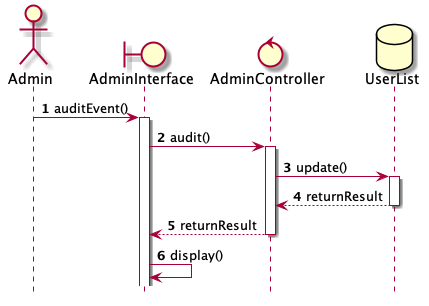
\includegraphics[width=12cm]{misc/figure_src/sequence_diagram/sd_audit_user.png}
% 		%     \caption{用户注册用例时序图}
% 		%     \label{fig:sd_auditUser}
% 		%     %\end{adjustwidth}
% 		% \end{figure}

% 	\end{enumerate}
% 	% subsection 用户查询用例分析 (end)

% 	\subsection{用户管理用例分析} % (fold)
% 	\label{sub:用户审核用例分析}
% 	\begin{enumerate}
% 		\item \textbf{类的析取} \\
% 		用户审核用例允许管理员处理微供应商和采购商提交的注册信息,管理员可以执行审核通过和审核不通过两种操作,其中包括的实体类、控制类和边界类如下图。
% 		\autoref{fig:class_auditUser}
% 		\begin{figure}[htp]
% 		    %\begin{adjustwidth}{-1.5cm}{-1cm}
% 		    \centering
% 		    
\includegraphics[width=12cm]{misc/figure_src/class_diagram/auditUser.png}
% 		    \caption{登录用例析取图}
% 		    \label{fig:class_auditUser}
% 		    %\end{adjustwidth}
% 		\end{figure}

% 		\item \textbf{用例工作时序图} \\
% 		在用户审核用例中,管理员在已经进行用户查询找到待审核用户后,可以在前端点击通过审核,审核确认信息由前端发送到后端,后端进行数据库操作后得到结果返回前端。具体流程如下图所示\autoref{fig:sd_auditUser}。

% 		\begin{figure}[htp]
% 		    %\begin{adjustwidth}{-1.5cm}{-1cm}
% 		    \centering
% 		    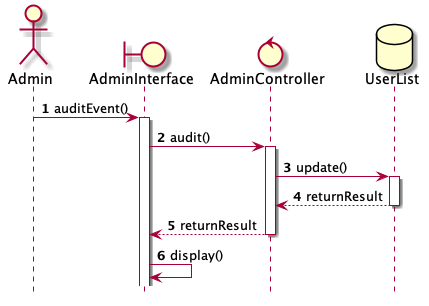
\includegraphics[width=12cm]{misc/figure_src/sequence_diagram/sd_audit_user.png}
% 		    \caption{用户管理用例时序图}
% 		    \label{fig:sd_auditUser}
% 		    %\end{adjustwidth}
% 		\end{figure}

% 	\end{enumerate}
% 	% subsection 用户审核用例分析 (end)

% 	\subsection{订单审核用例分析} % (fold)
% 	\label{sub:订单审核用例分析}
% 	\begin{enumerate}
% 		\item \textbf{类的析取} \\
% 		订单审核用例允许管理员审核来自采购商的订单申请和微供应商的更新子订单进度的申请,其中包括的实体类、控制类和边界类如下图。
% 		\autoref{fig:class_auditOrder}
% 		\begin{figure}[htp]
% 		    %\begin{adjustwidth}{-1.5cm}{-1cm}
% 		    \centering
% 		    
\includegraphics[width=12cm]{misc/figure_src/class_diagram/auditOrder.png}
% 		    \caption{登录用例析取图}
% 		    \label{fig:class_auditOrder}
% 		    %\end{adjustwidth}
% 		\end{figure}

% 		\item \textbf{用例工作时序图} \\
% 		在用户审核用例中,管理员在已经进行订单查询找到待审核用户后,可以在前端点击通过审核,审核确认信息由前端发送到后端,后端进行数据库操作后得到结果返回前端。具体流程如下图所示\autoref{fig:sd_auditOrder}

% 		\begin{figure}[htp]
% 		    %\begin{adjustwidth}{-1.5cm}{-1cm}
% 		    \centering
% 		    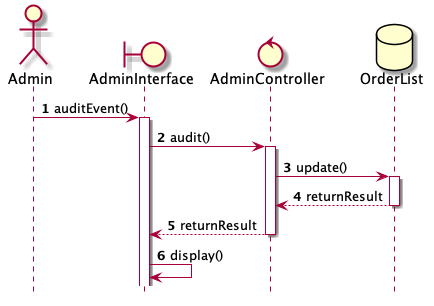
\includegraphics[width=12cm]{misc/figure_src/sequence_diagram/sd_audit_order.png}
% 		    \caption{用户注册用例时序图}
% 		    \label{fig:sd_auditOrder}
% 		    %\end{adjustwidth}
% 		\end{figure}
% 	\end{enumerate}

\newpage
	\subsection{订单加入用例分析} % (fold)
	\label{sub:订单加入用例分析}
	\begin{enumerate}
		\item \textbf{类的析取} \\
		订单加入用例允许微供应商在查询了母订单后加入某母订单,并在数据库中生成对应的子订单信息,其中包括的实体类、控制类和边界类如下图
		\autoref{fig:class_join}。
		\begin{figure}[htp]
		    %\begin{adjustwidth}{-1.5cm}{-1cm}
		    \centering
		    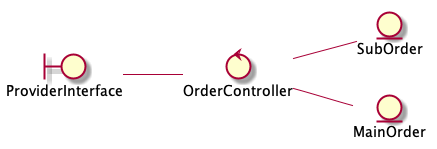
\includegraphics[width=12cm]{report/figure/classAnalyse/join.png}
		    \caption{订单加入用例析取图}
		    \label{fig:class_join}
		    %\end{adjustwidth}
		\end{figure}

		\item \textbf{用例工作时序图} \\
		在订单加入用例中,微供应商在已经查询了母订单信息后可以选择合适的母订单加入,在前端点击“加入”后,该信息发送到后端并生成子订单信息并修改母订单。具体流程如下图所示\autoref{fig:sd_joinOrder}

		\begin{figure}[htp]
		    %\begin{adjustwidth}{-1.5cm}{-1cm}
		    \centering
		    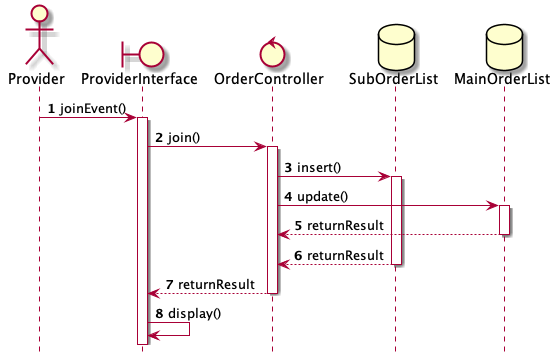
\includegraphics[width=12cm]{report/figure/sequenceDiagram/sd_joinOrder.png}
		    \caption{订单加入用例工作时序图}
		    \label{fig:sd_joinOrder}
		    %\end{adjustwidth}
		\end{figure}
	\end{enumerate}
	
	% subsection 订单加入用例分析 (end)

\section{分析机制} 
	根据 1.4 补充规约得到上述边界类、控制类、实体类需要满足的非功能性需求, 列出系统的分析机制表,如下表所示:

	\begin{table}[h]
		\centering
		\caption{”鲜天下“平台分析机制}
		\begin{tabular}{|c|c|}
			\hline  
				分析类 & 分析机制性\\
			\hline  
				User & 持久性、安全性\\
			\hline  
				MainOrder & 持久性、安全性\\
			\hline
				SubOrder & 持久性、安全性\\
			\hline  
				UserInterface & 持久性、遗留接口\\
			\hline
				UserController & 分布式\\
			\hline
		\end{tabular}
	\end{table}



\section{合并分析类}

% TODO: 类图

	将析取出来的边界类、控制类、实体类进行合并整理,得到的系统的合并类图如下图所示:\\
	\begin{figure}[htp]
		    \begin{adjustwidth}{-1cm}{-1cm}
		    \centering
		    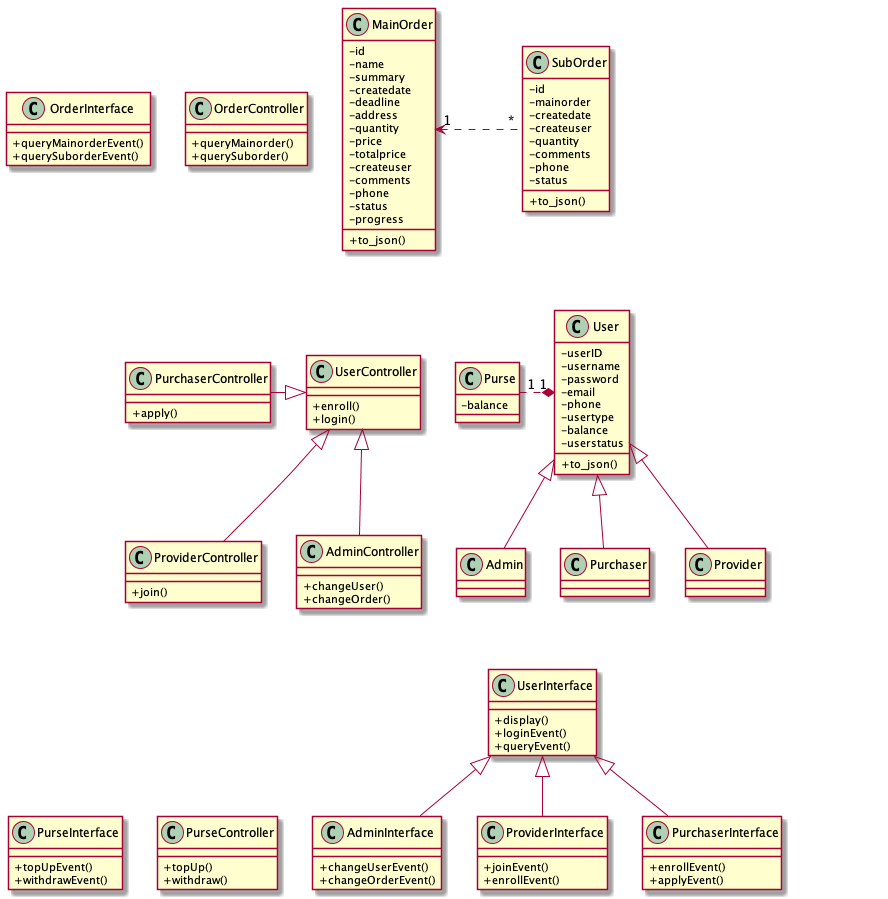
\includegraphics[width=20cm]{report/figure/class_system.png}
		    \caption{“鲜天下”平台合并类图}
		    % \label{fig:class_join}
		    \end{adjustwidth}
		\end{figure}
